\documentclass[11pt,a4paper]{article}
\usepackage[
    left=0.73in,
    right=0.73in,
    top=.8in,
    bottom=.50in,
    paperheight=11in,
    paperwidth=8.5in
]{geometry}

\usepackage{graphicx}

\begin{document}
% Cover Page
\pagenumbering{gobble}
\begin{center}
\textbf{
    \Large{ECE 543: Introduction to Digital Systems}
    \\~\\
    \large{Instructor: Bessam Zuhair Al Jewad, Ph.D.}
    \\[1.25in]
    \LARGE{Prelab \#8: Synchronous Sequential Logic Design}
    \\[0.62in]
    \large{Prepared for Himadri Basu (TA)\\~\\By Christopher Chin}
    \\[1.25in]
    \LARGE{Section 6}
    \\[1.25in]
    \Large{Department of Electrical and Computer Engineering\\
           University of New Hampshire}
    \\[1.25in]
    \Large{\today}
}
\end{center}
\clearpage
\pagenumbering{arabic}

% TOC
\tableofcontents
\pagebreak

% Pages
\section{Introduction}
The objective of this lab is to design, assemble, and test a synchronous sequential logic circuit.
\section{Equipment Required}
    \item Global Specialties Design and Prototyping PB-505
    \item Wire leads
    \item Logic Probe (1)
    \item 7400 TTL Quad Two Input NAND gate Integrated Circuit (2)
    \item 7408 TTL Quad Two Input AND gate Integrated Circuit (1)
    \item 7410 TTL Triple Input NAND gate Integrated Circuit (2)
    \item 74175 TTL Quad D Positive Edge-Triggered Flip-Flop Integrated Circuit (1)
\section{Procedure}
\begin{figure}[h]
    \centering
    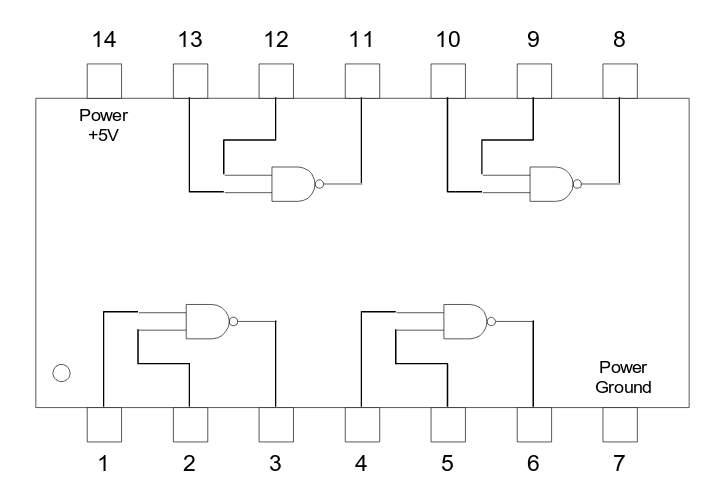
\includegraphics[width=5in]{IC.png}
    \caption{IC7400 Circuit Diagram}
\end{figure}7400
\section{Appendix}
\section{References}
Ronald J. Tocci et al. 2011. Digital Systems: Principles and Applications, 11\textsuperscript{th} Ed.

\end{document}
